\chapter{SYSTEM EVALUATION \& DESIGN}
\section{Introduction}
Research works in the arena of modern web applications emphasize the transition from monolithic structures to highly scalable, component-driven architectures. To overcome the limitations of legacy e-commerce systems—such as slow loading times, poor state management, and complex user interfaces—we have proposed and developed "GloBus" using the MERN stack (MongoDB, Express.js, React.js, Node.js). In this chapter, we evaluate the system requirements, present our chosen software development methodology, and provide comprehensive design diagrams (ERD, DFD, Use Case) that define the architectural blueprint of GloBus. Finally, we showcase the core features implemented within the platform.

\section{Requirement Analysis}
E-commerce has evolved over the last decade from being a supplementary retail tool to becoming the primary backbone of global trade. The initial focus of our research was to identify the pain points of existing platforms in Bangladesh. Based on user feedback and market analysis, we developed system conditions for a purpose-built digital marketplace. These findings led us to design GloBus with a focus on speed (React + Vite), localized secure payments (SSLCommerz), and advanced search capabilities (AI Vision). The system requirements are broadly categorized into non-functional and functional requirements.

\subsection{Non-Functional Requirements}
Requirement Analysis, also known as Requirement Engineering, is the process of defining user expectations for a new software being built. Non-functional requirements dictate the system's operational capabilities and constraints rather than specific behaviors. For GloBus, the critical non-functional demands include:
\begin{itemize}
    \item \textbf{Usability Demand:} The system must have an intuitive interface with seamless navigation (e.g., Dark/Light mode, multi-language support).
    \item \textbf{Performance \& Capacity Demand:} The frontend must load quickly even on mid-range devices, managed efficiently by Vite and React's virtual DOM.
    \item \textbf{Security Demand:} High security for user data and passwords using Bcrypt and JWT authentication.
    \item \textbf{Data Integrity Demand:} Accurate real-time syncing of the shopping cart and inventory database.
    \item \textbf{Availability Demand:} The system architecture should support continuous uptime.
    \item \textbf{Manageability Demand:} A robust admin panel for effortless management of the platform.
\end{itemize}

\subsection{Functional Requirements}
A Functional Requirement (FR) is a description of the service that the software must offer. It describes specific functionalities which define what the system is expected to perform.

Functional Requirements of GloBus include:
\begin{itemize}
    \item User Registration (Sign Up) and Secure Sign In.
    \item Browse and Search Products by category, keyword, or AI Vision (Image Search).
    \item Add items to the Shopping Cart and manage cart quantities.
    \item Add favorite items to a Wishlist.
    \item Secure multi-step Checkout process with delivery information.
    \item Process payments securely via SSLCommerz.
    \item View Order History and Track Order Status.
    \item Admin ability to Add, Update, and Delete Products (CRUD).
    \item Admin ability to view, manage, and update Order statuses.
    \item Admin ability to manage Users (Ban, Update Role).
    \item Newsletter Subscription.
\end{itemize}

\section{Methodology}
\subsection{Agile Development Model}
We chose the Agile Development model for our project. Agile is a faster, highly iterative way to develop software. It is a people- and result-focused methodology that is highly flexible and makes it easy to improve software quality progressively. It works on the principle of fast and incremental delivery.

\begin{figure}[h]
\centering
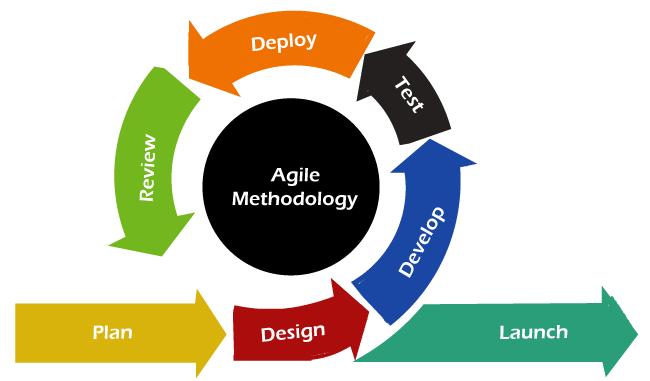
\includegraphics[width=\textwidth]{images/Agile.png}
\caption{Agile Development Model}
\end{figure}

Reasons for choosing Agile Development for GloBus:
\begin{itemize}
    \item Allows for continuous integration of complex features (like AI Vision and SSLCommerz) in sprints.
    \item Faster releases and continuous testing of individual components (React components).
    \item Greater project transparency and easy adaptation to changing requirements.
    \item Competitive advantage achieved by spotting defects (e.g., cart syncing issues) early in the development process rather than at the end.
\end{itemize}

\subsection{Gantt Chart}
A Gantt chart is a visual view of tasks scheduled over time. It represents the project timeline, showing the start and finish dates of the terminal elements and summary elements of the GloBus project, from initial requirement analysis and UI design to backend development and final deployment.

\begin{figure}[h]
\centering
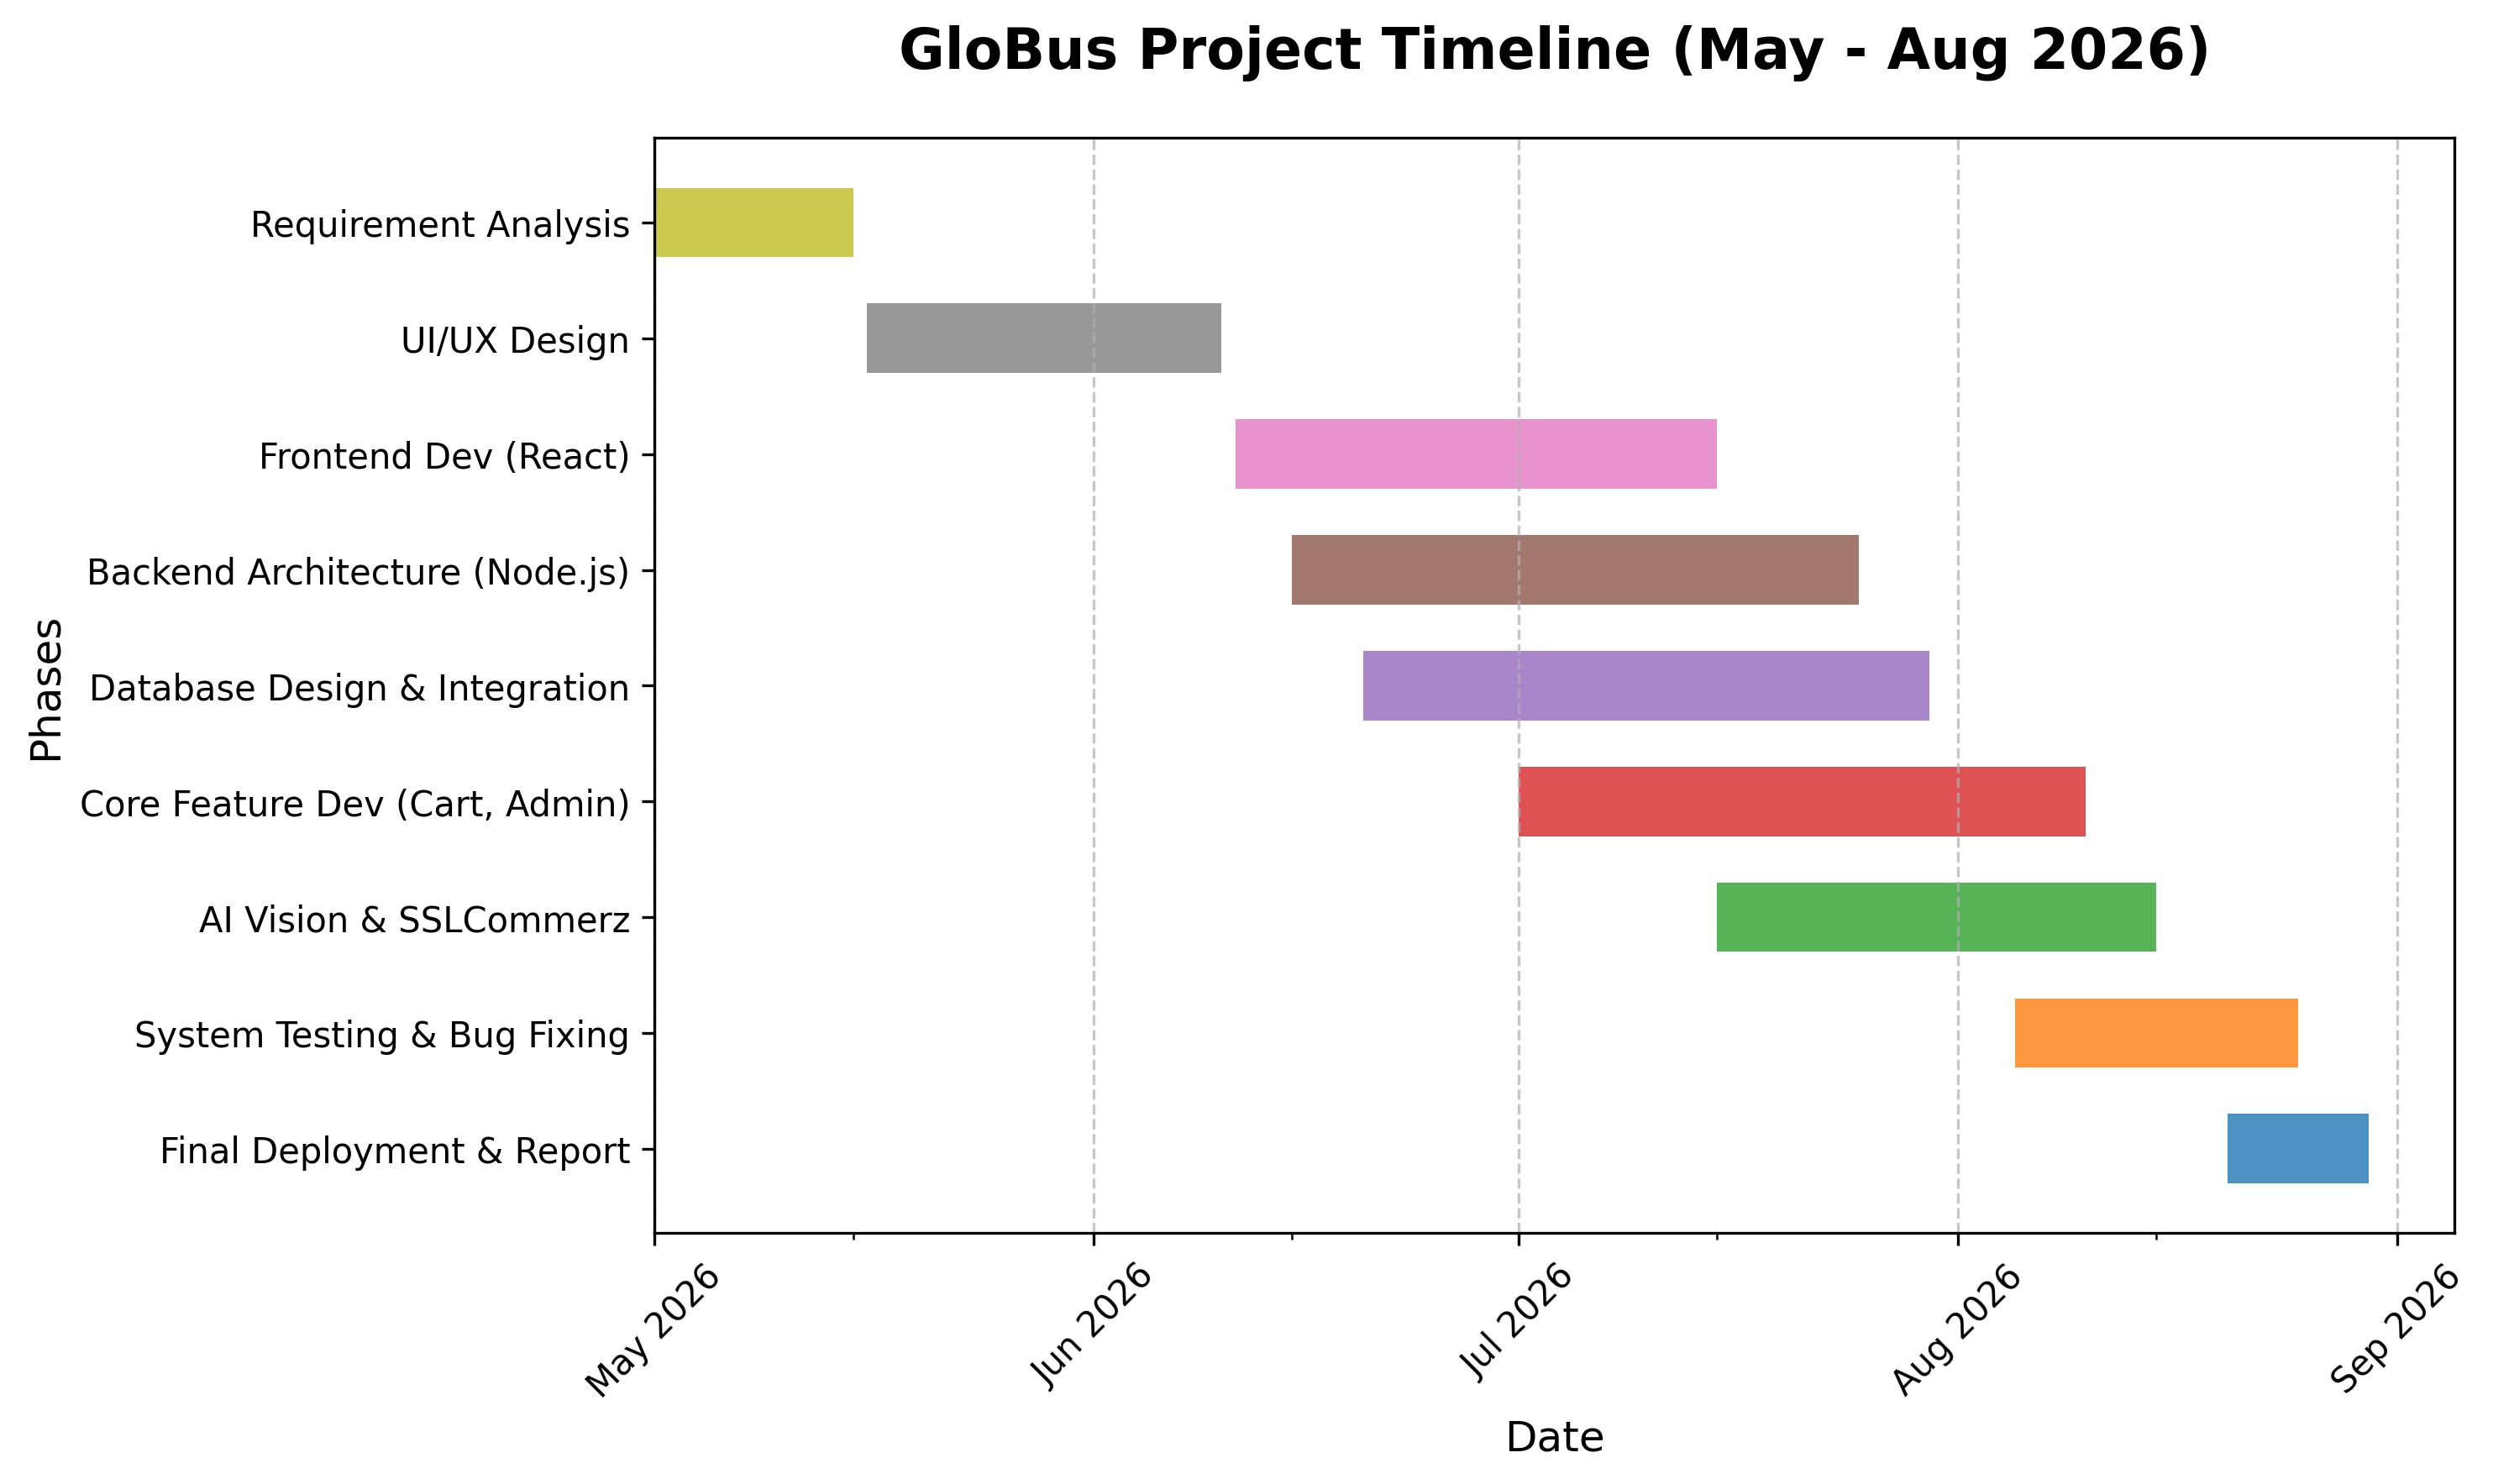
\includegraphics[width=\textwidth]{images/gantt.png}
\caption{Project Gantt Chart}
\end{figure}

\section{System Architecture Diagrams}
\subsection{Data Flow Diagram (DFD)}
Data Flow Diagrams provide a graphical representation of the flow of data through an information system, modeling its process aspects. 

\textbf{Context Level DFD:} The Context Level DFD represents the entire GloBus system as a single high-level process interacting with external entities. The primary external entities include the Customer (who browses and purchases), the Administrator (who manages inventory), and the Payment Gateway (SSLCommerz, which verifies transactions).

\begin{figure}[h]
\centering
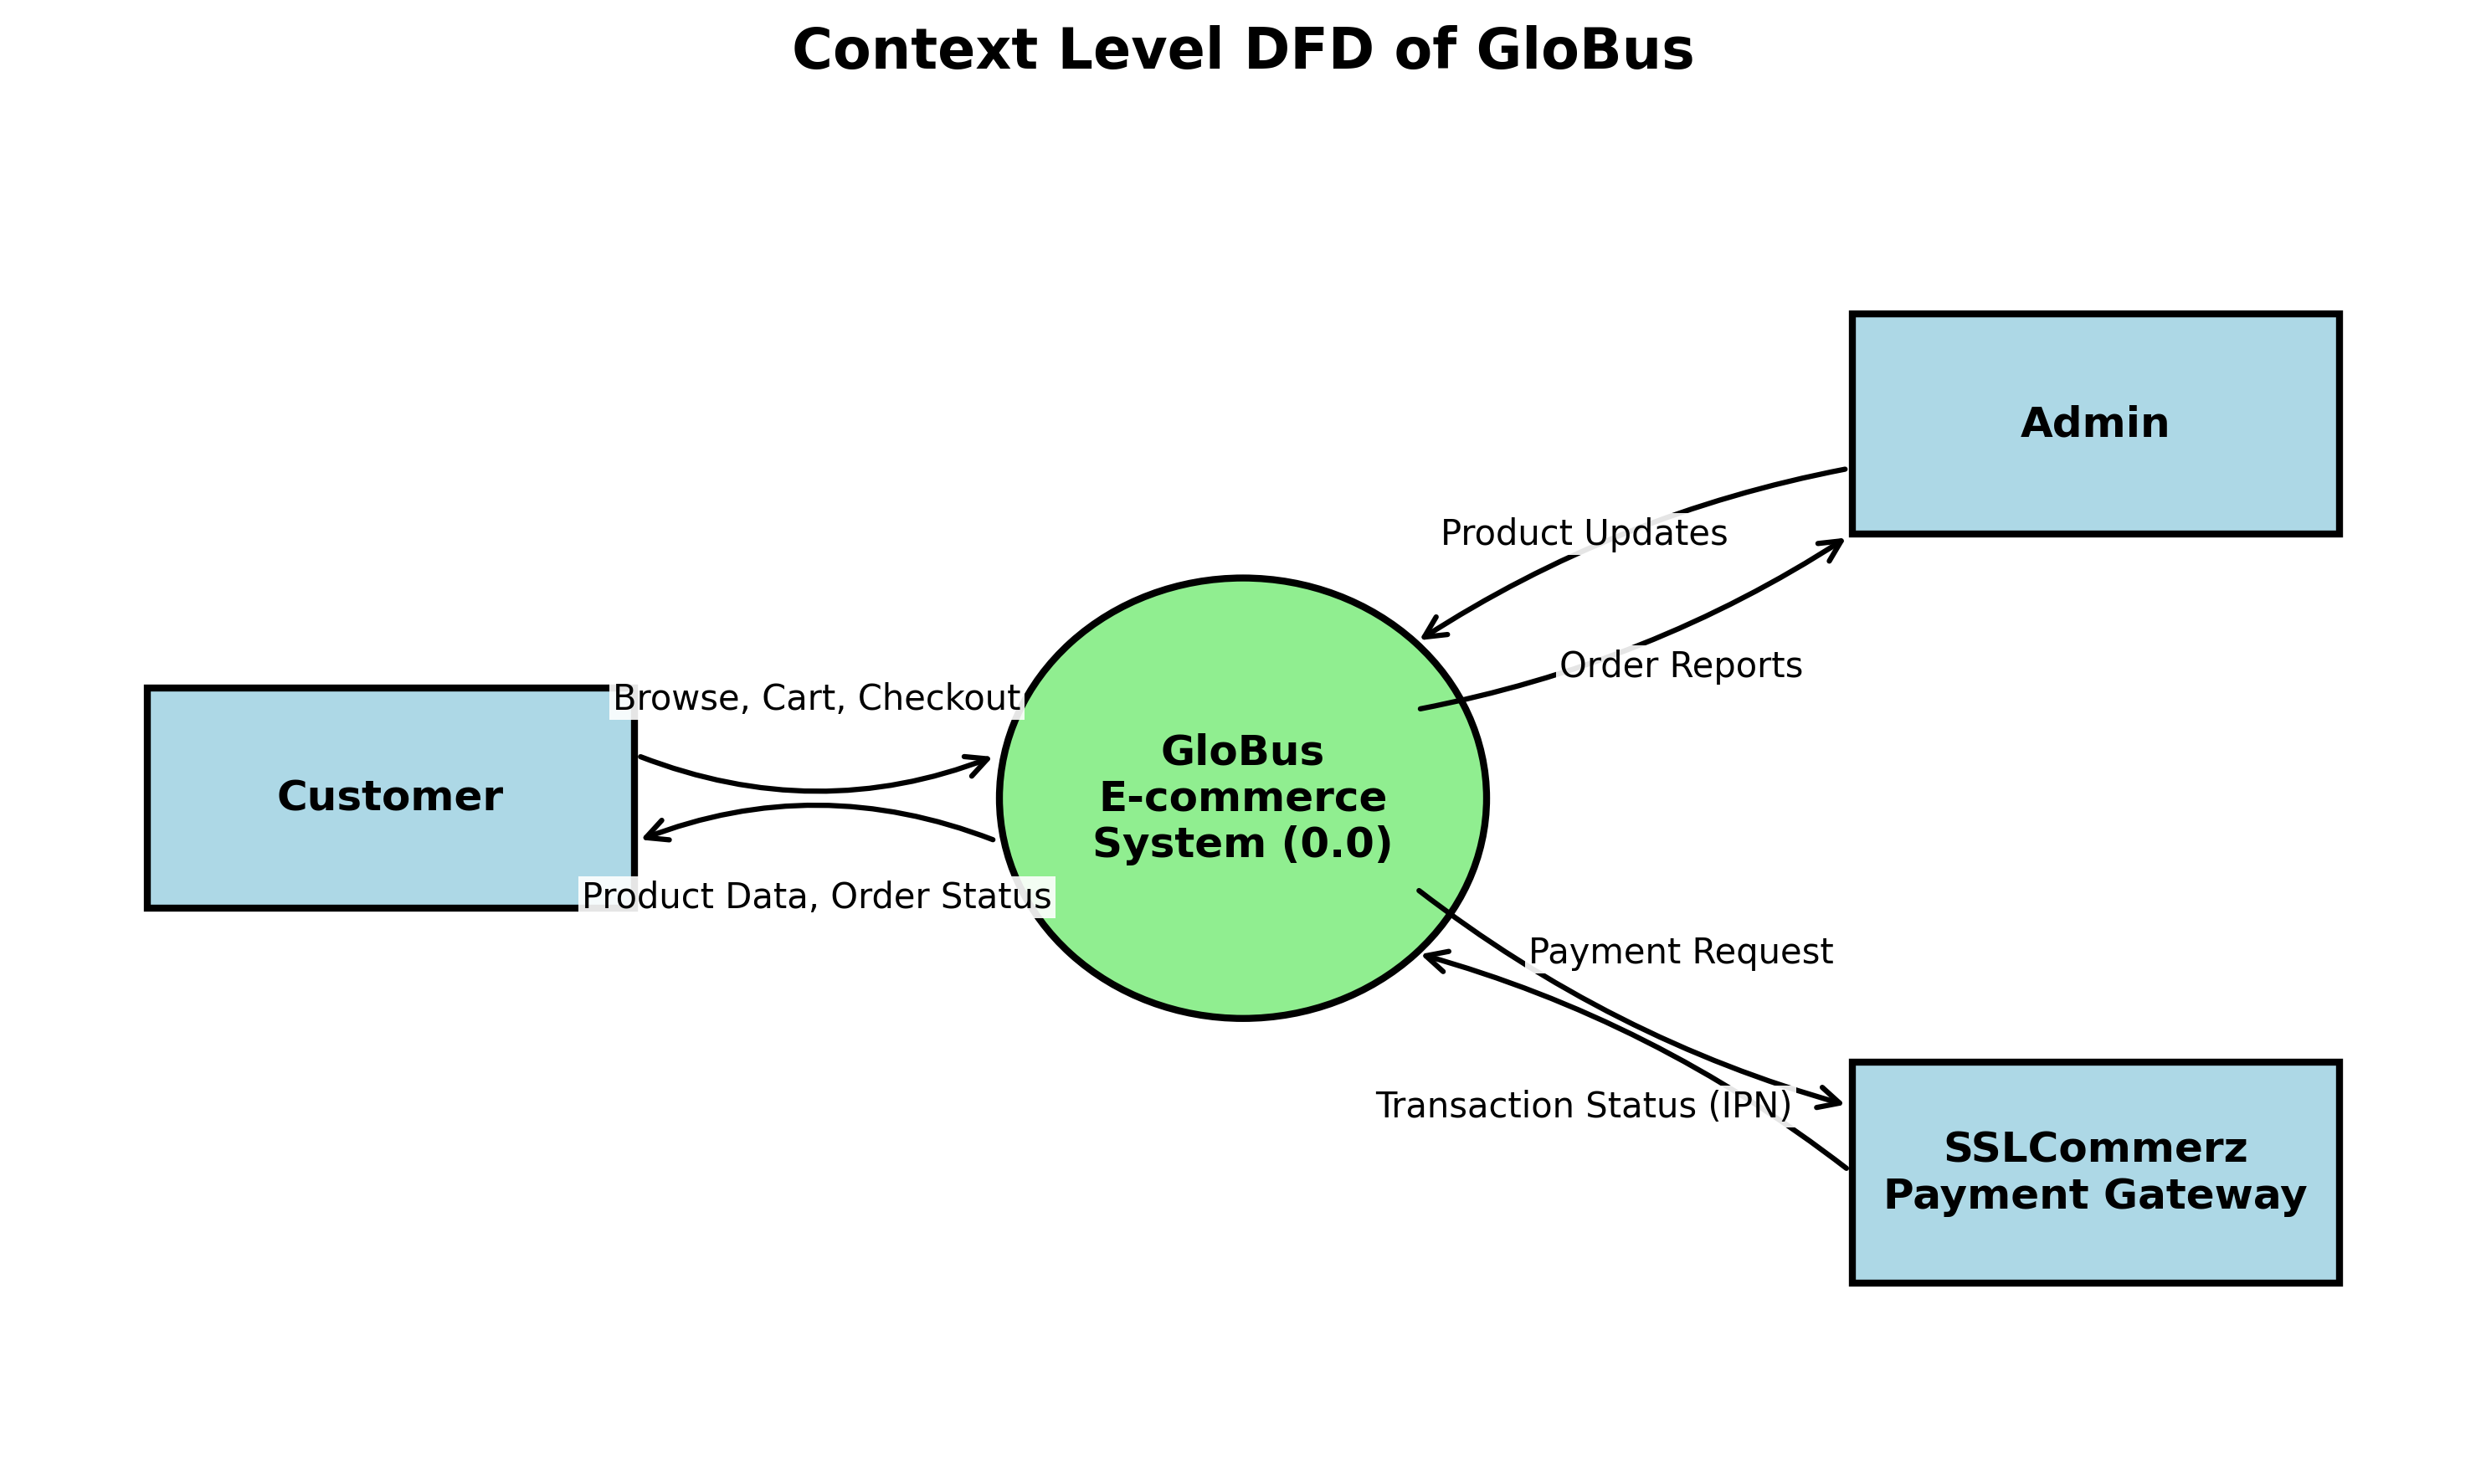
\includegraphics[width=\textwidth]{images/dfd_context.png}
\caption{Context Level DFD of GloBus}
\end{figure}

\textbf{Level-0 DFD:} The Level-0 DFD breaks down the context diagram into major sub-processes. It illustrates how data flows between critical modules such as the Authentication System, Product Management, Shopping Cart, and Order Processing, providing a deeper look into the system's internal data routing and data stores (MongoDB).

\begin{figure}[h]
\centering
\includegraphics[width=\textwidth]{images/dfd_level0.png}
\caption{Level-0 DFD of GloBus}
\end{figure}

\subsection{Entity Relationship (ER) Diagram}
The ER Diagram outlines the logical structure of the database. For GloBus, it maps out the primary entities (Users, Products, Orders, Cart, Categories, Reviews) and their relationships. For instance, it displays the one-to-many relationship between a User and their Orders, and the many-to-many relationship between Orders and Products, serving as the blueprint for our MongoDB schema.

\begin{figure}[h]
\centering
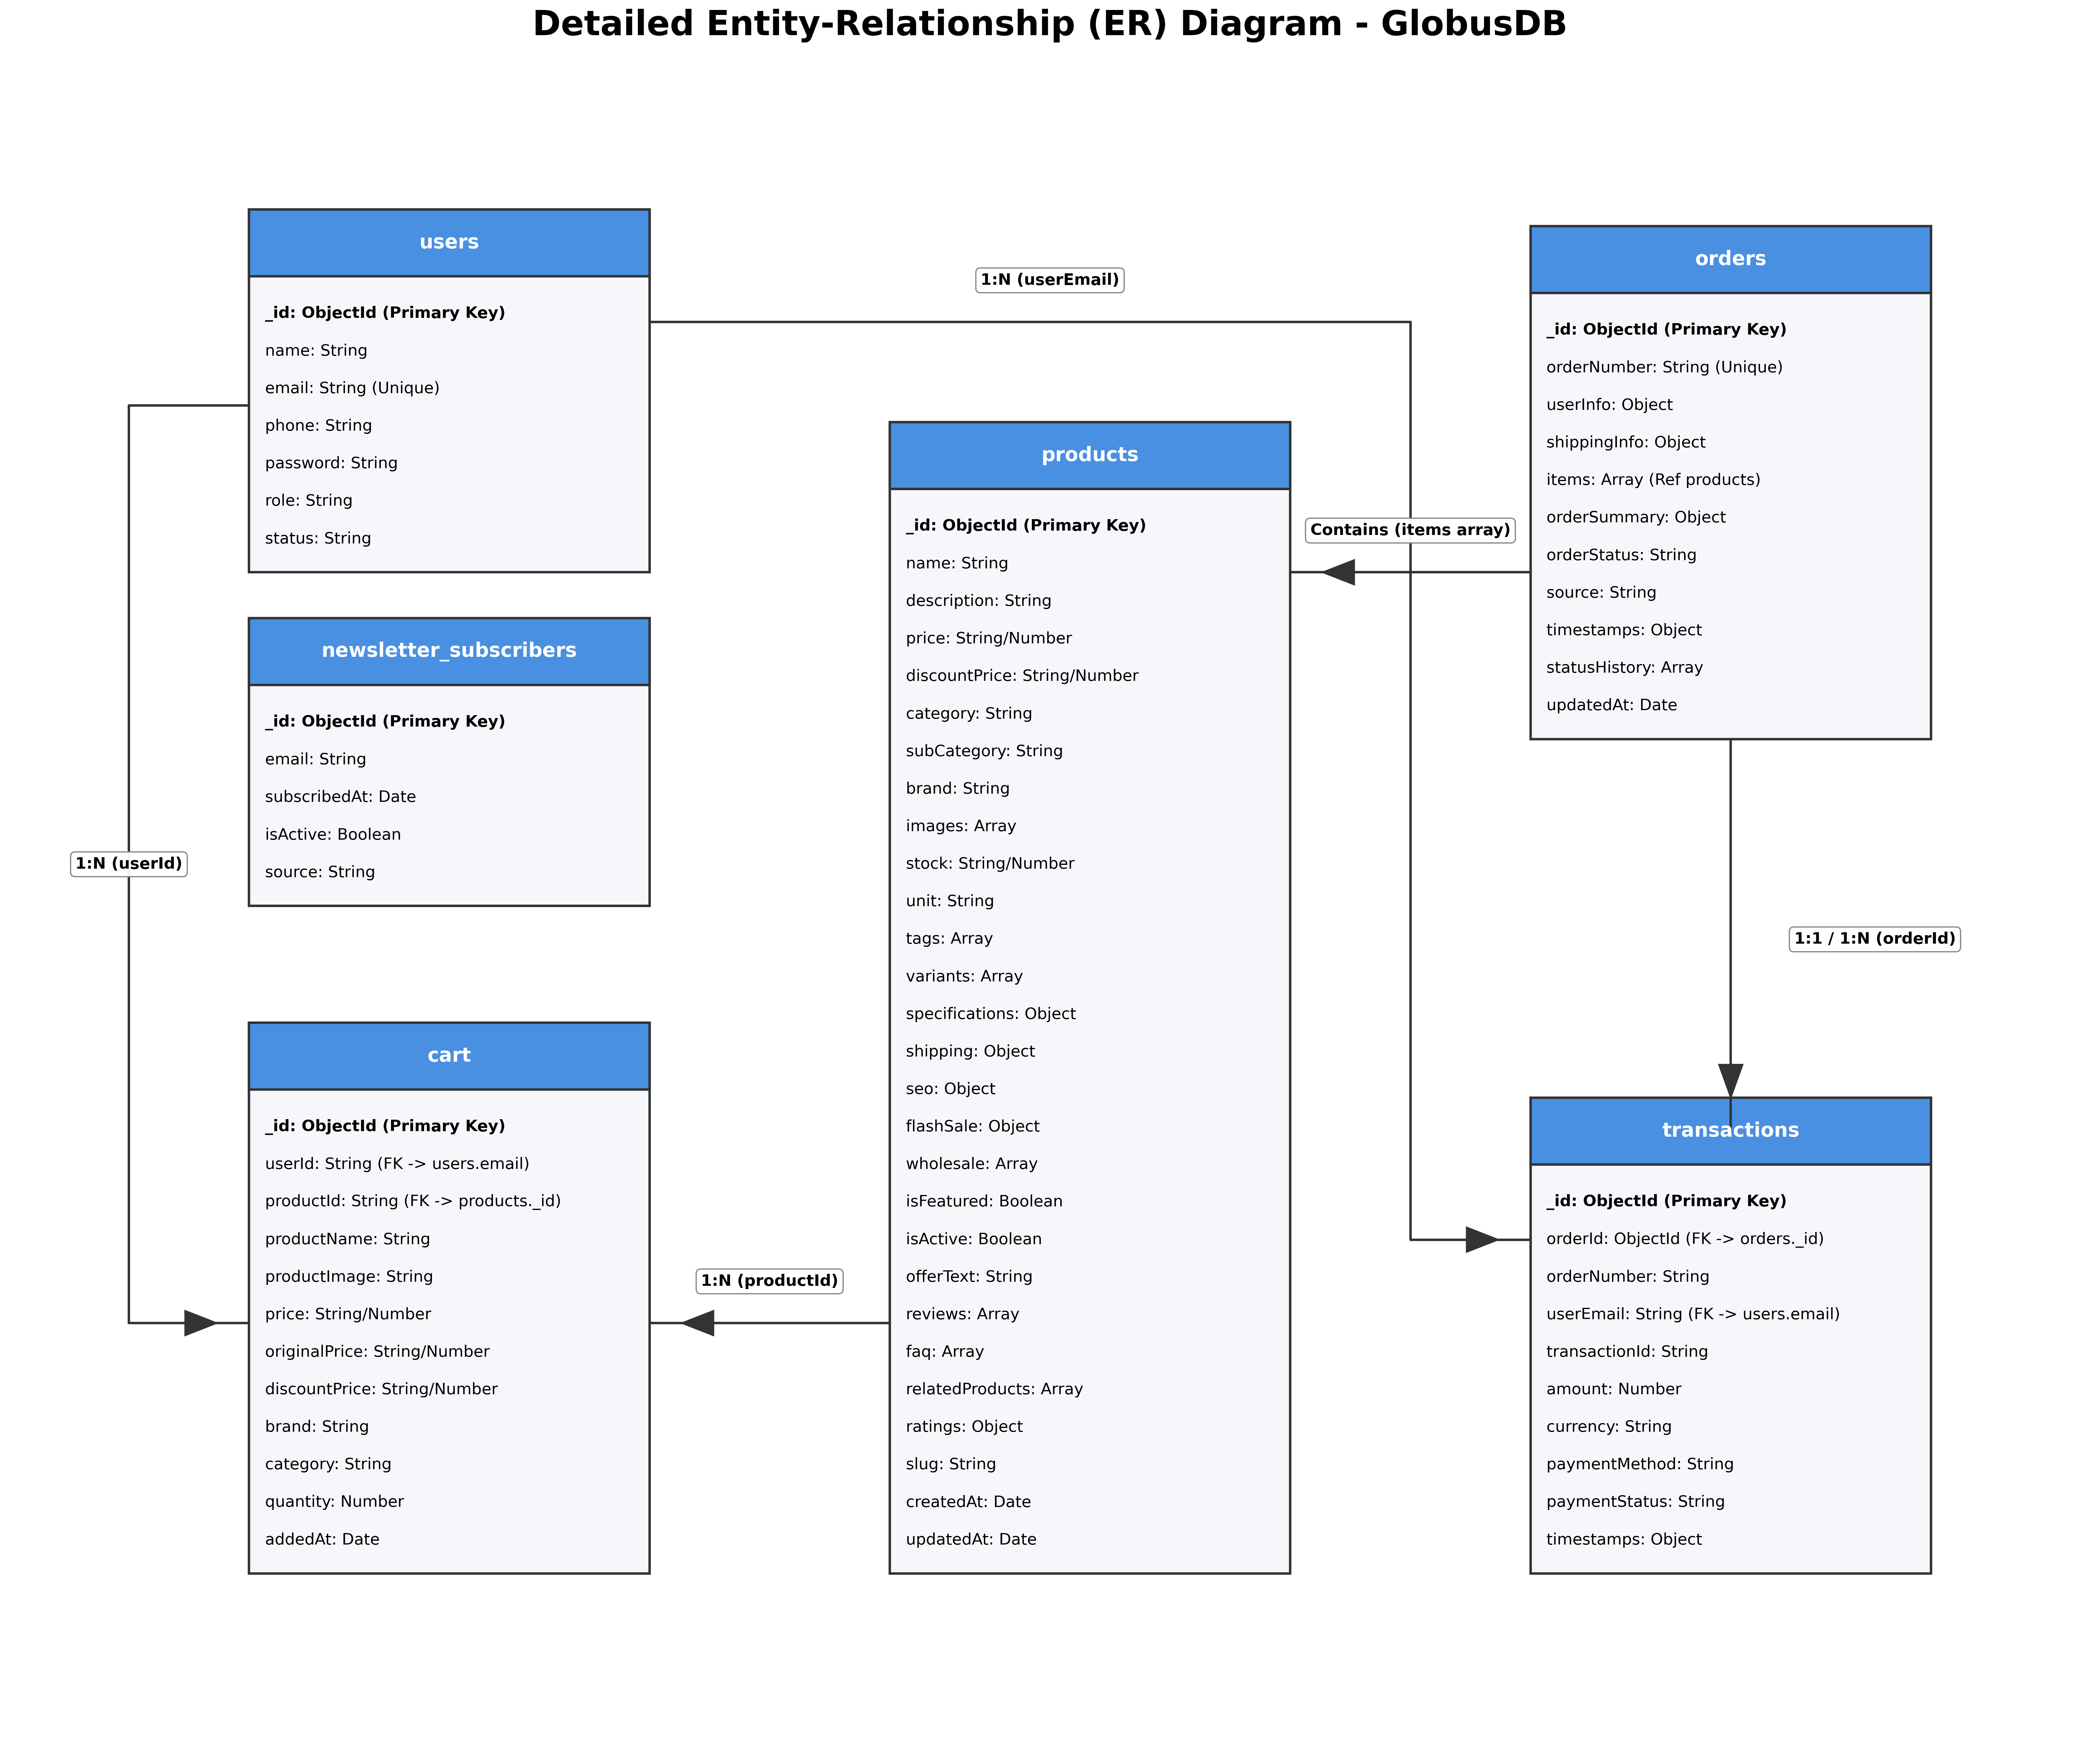
\includegraphics[width=\textwidth]{images/er_diagram.png}
\caption{ER Diagram of GloBus Database}
\end{figure}

\subsection{Use Case Diagram}
The Use Case Diagram visualizes the functional requirements of the system from the users' perspective. It defines the primary actors (Customer, Admin, Guest) and the various use cases they can perform. For example, it illustrates how a Customer can "Add to Cart" or "Checkout", while an Admin can "Manage Inventory" and "Update Order Status".

\begin{figure}[h]
\centering
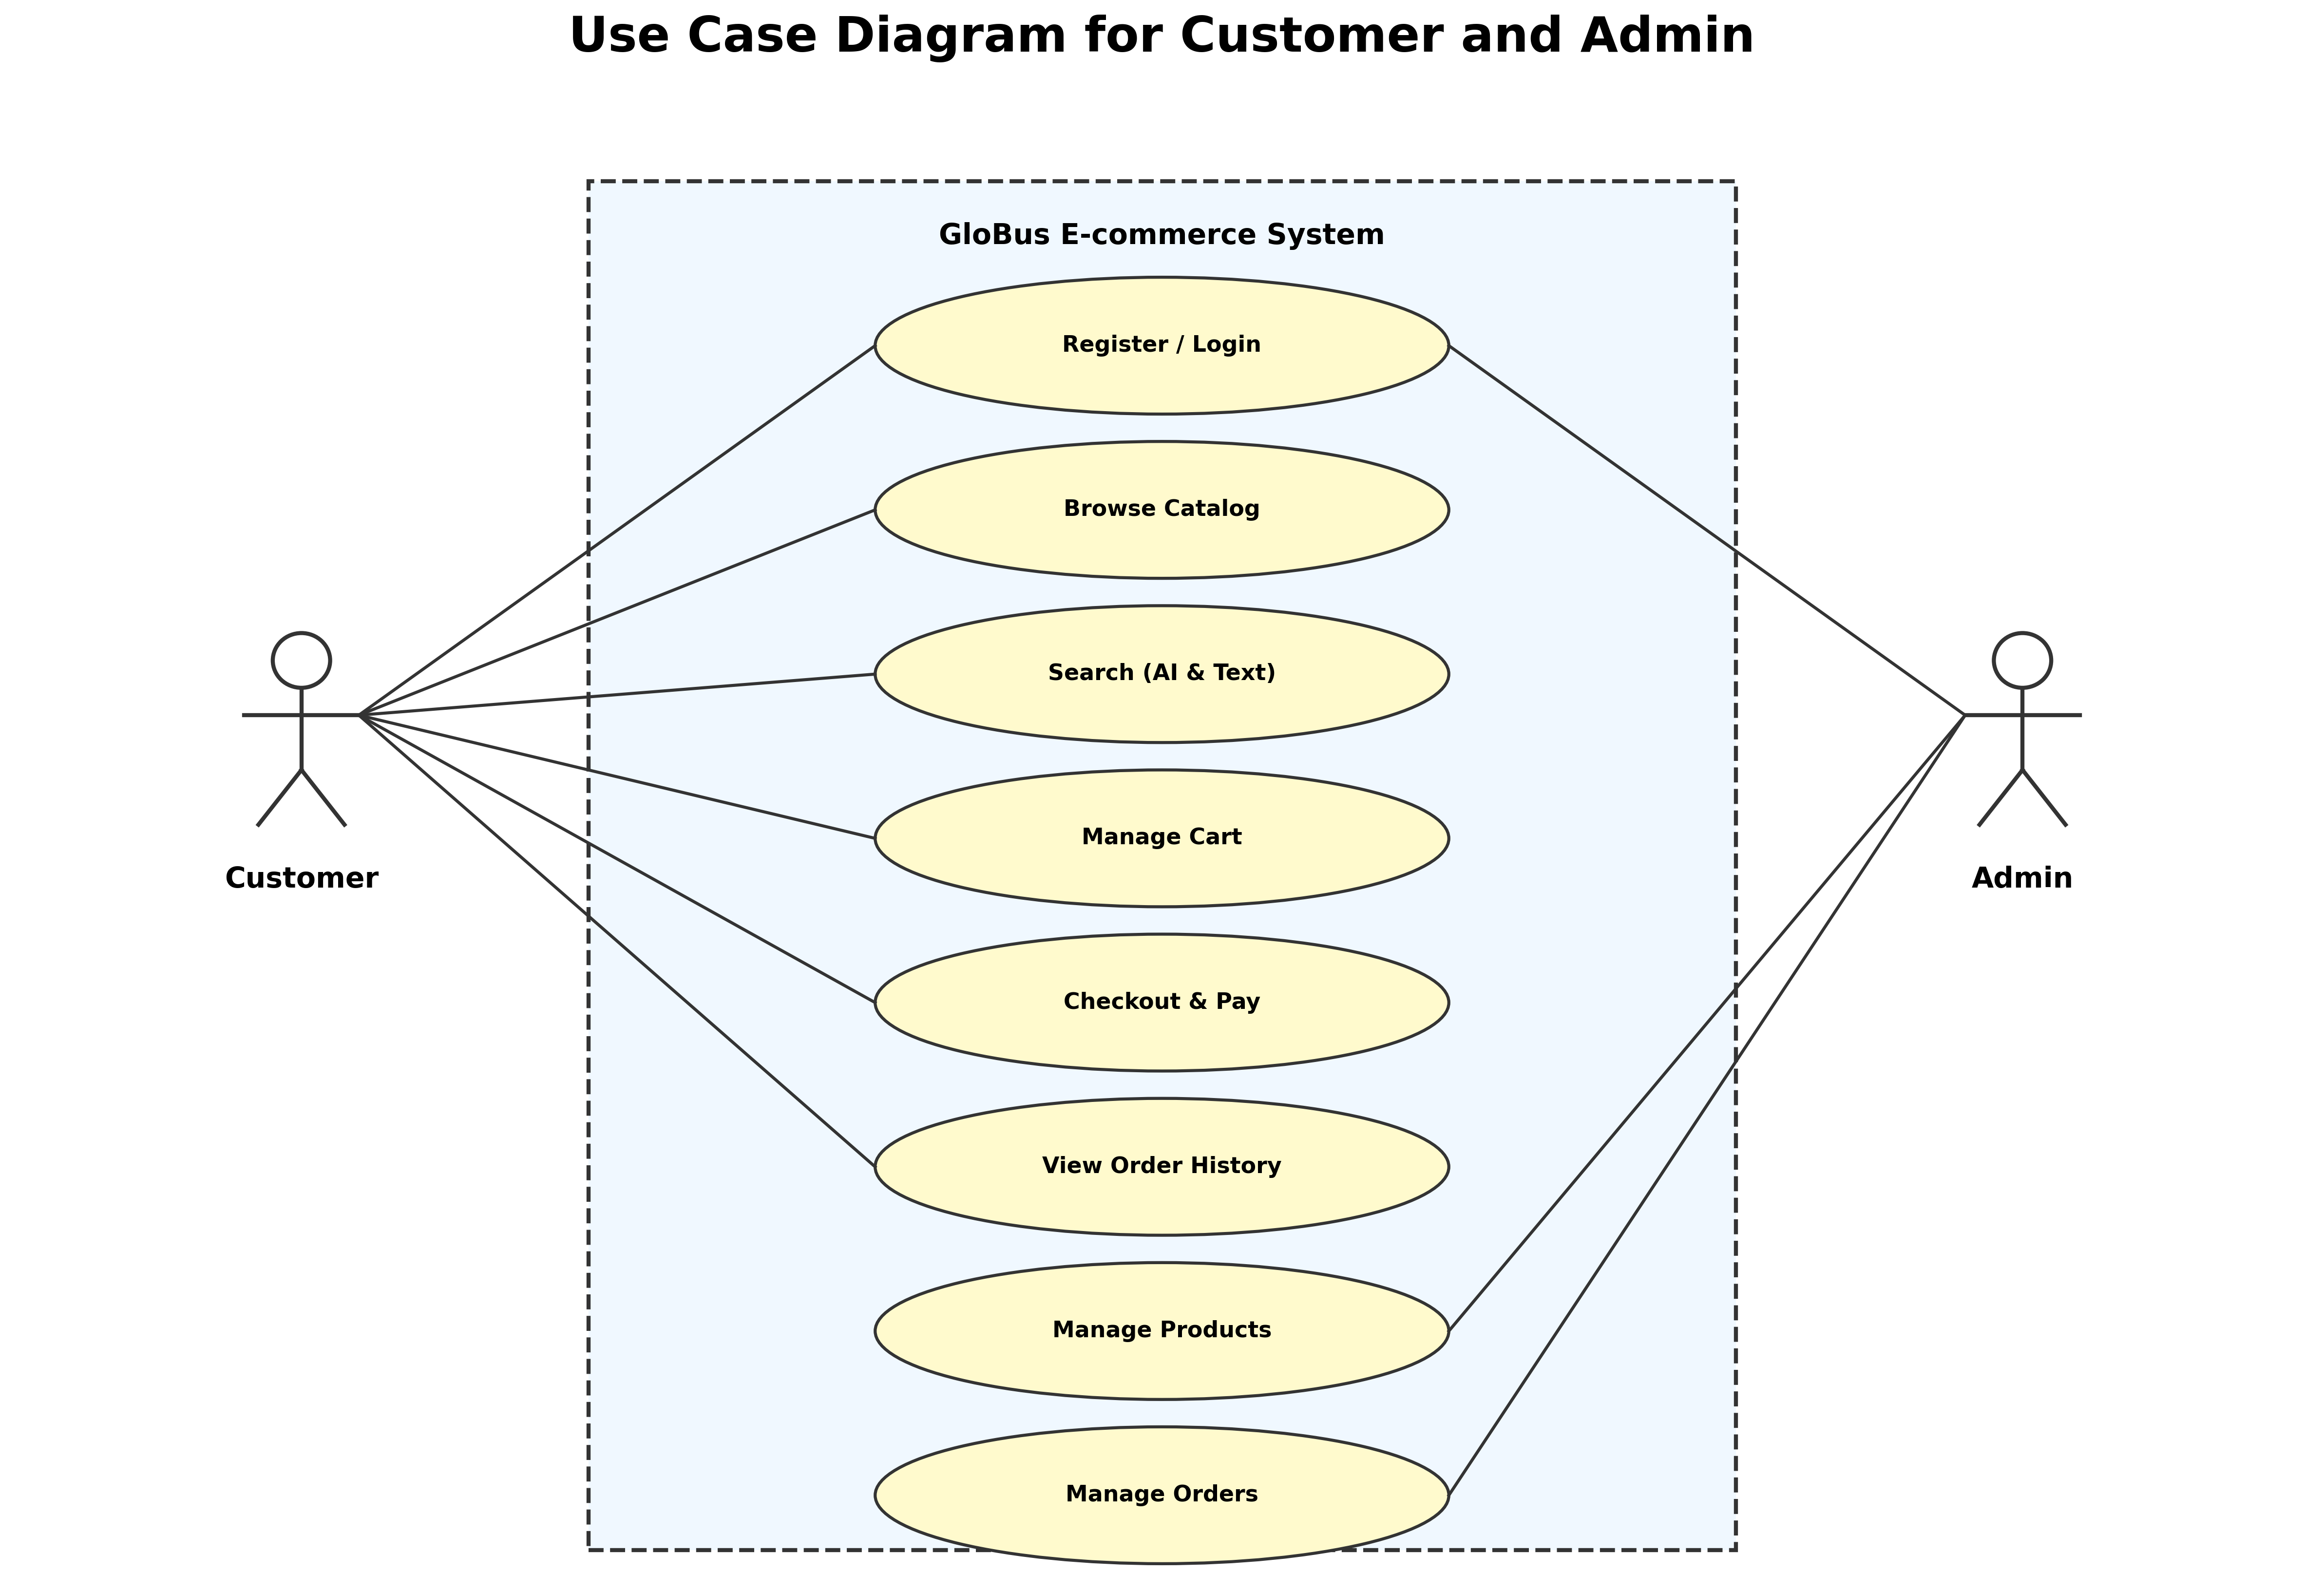
\includegraphics[width=\textwidth]{images/use_case.png}
\caption{Use Case Diagram for Customer and Admin}
\end{figure}

\subsection{Activity Diagram}
The Activity Diagram represents the flow of control or object flow within the system. The depicted diagram focuses on the core Checkout Process. It illustrates the sequential decision-making steps a user takes: from verifying their cart, entering shipping details, selecting a payment method, to confirming the transaction and generating the final order invoice.

\begin{figure}[h]
\centering
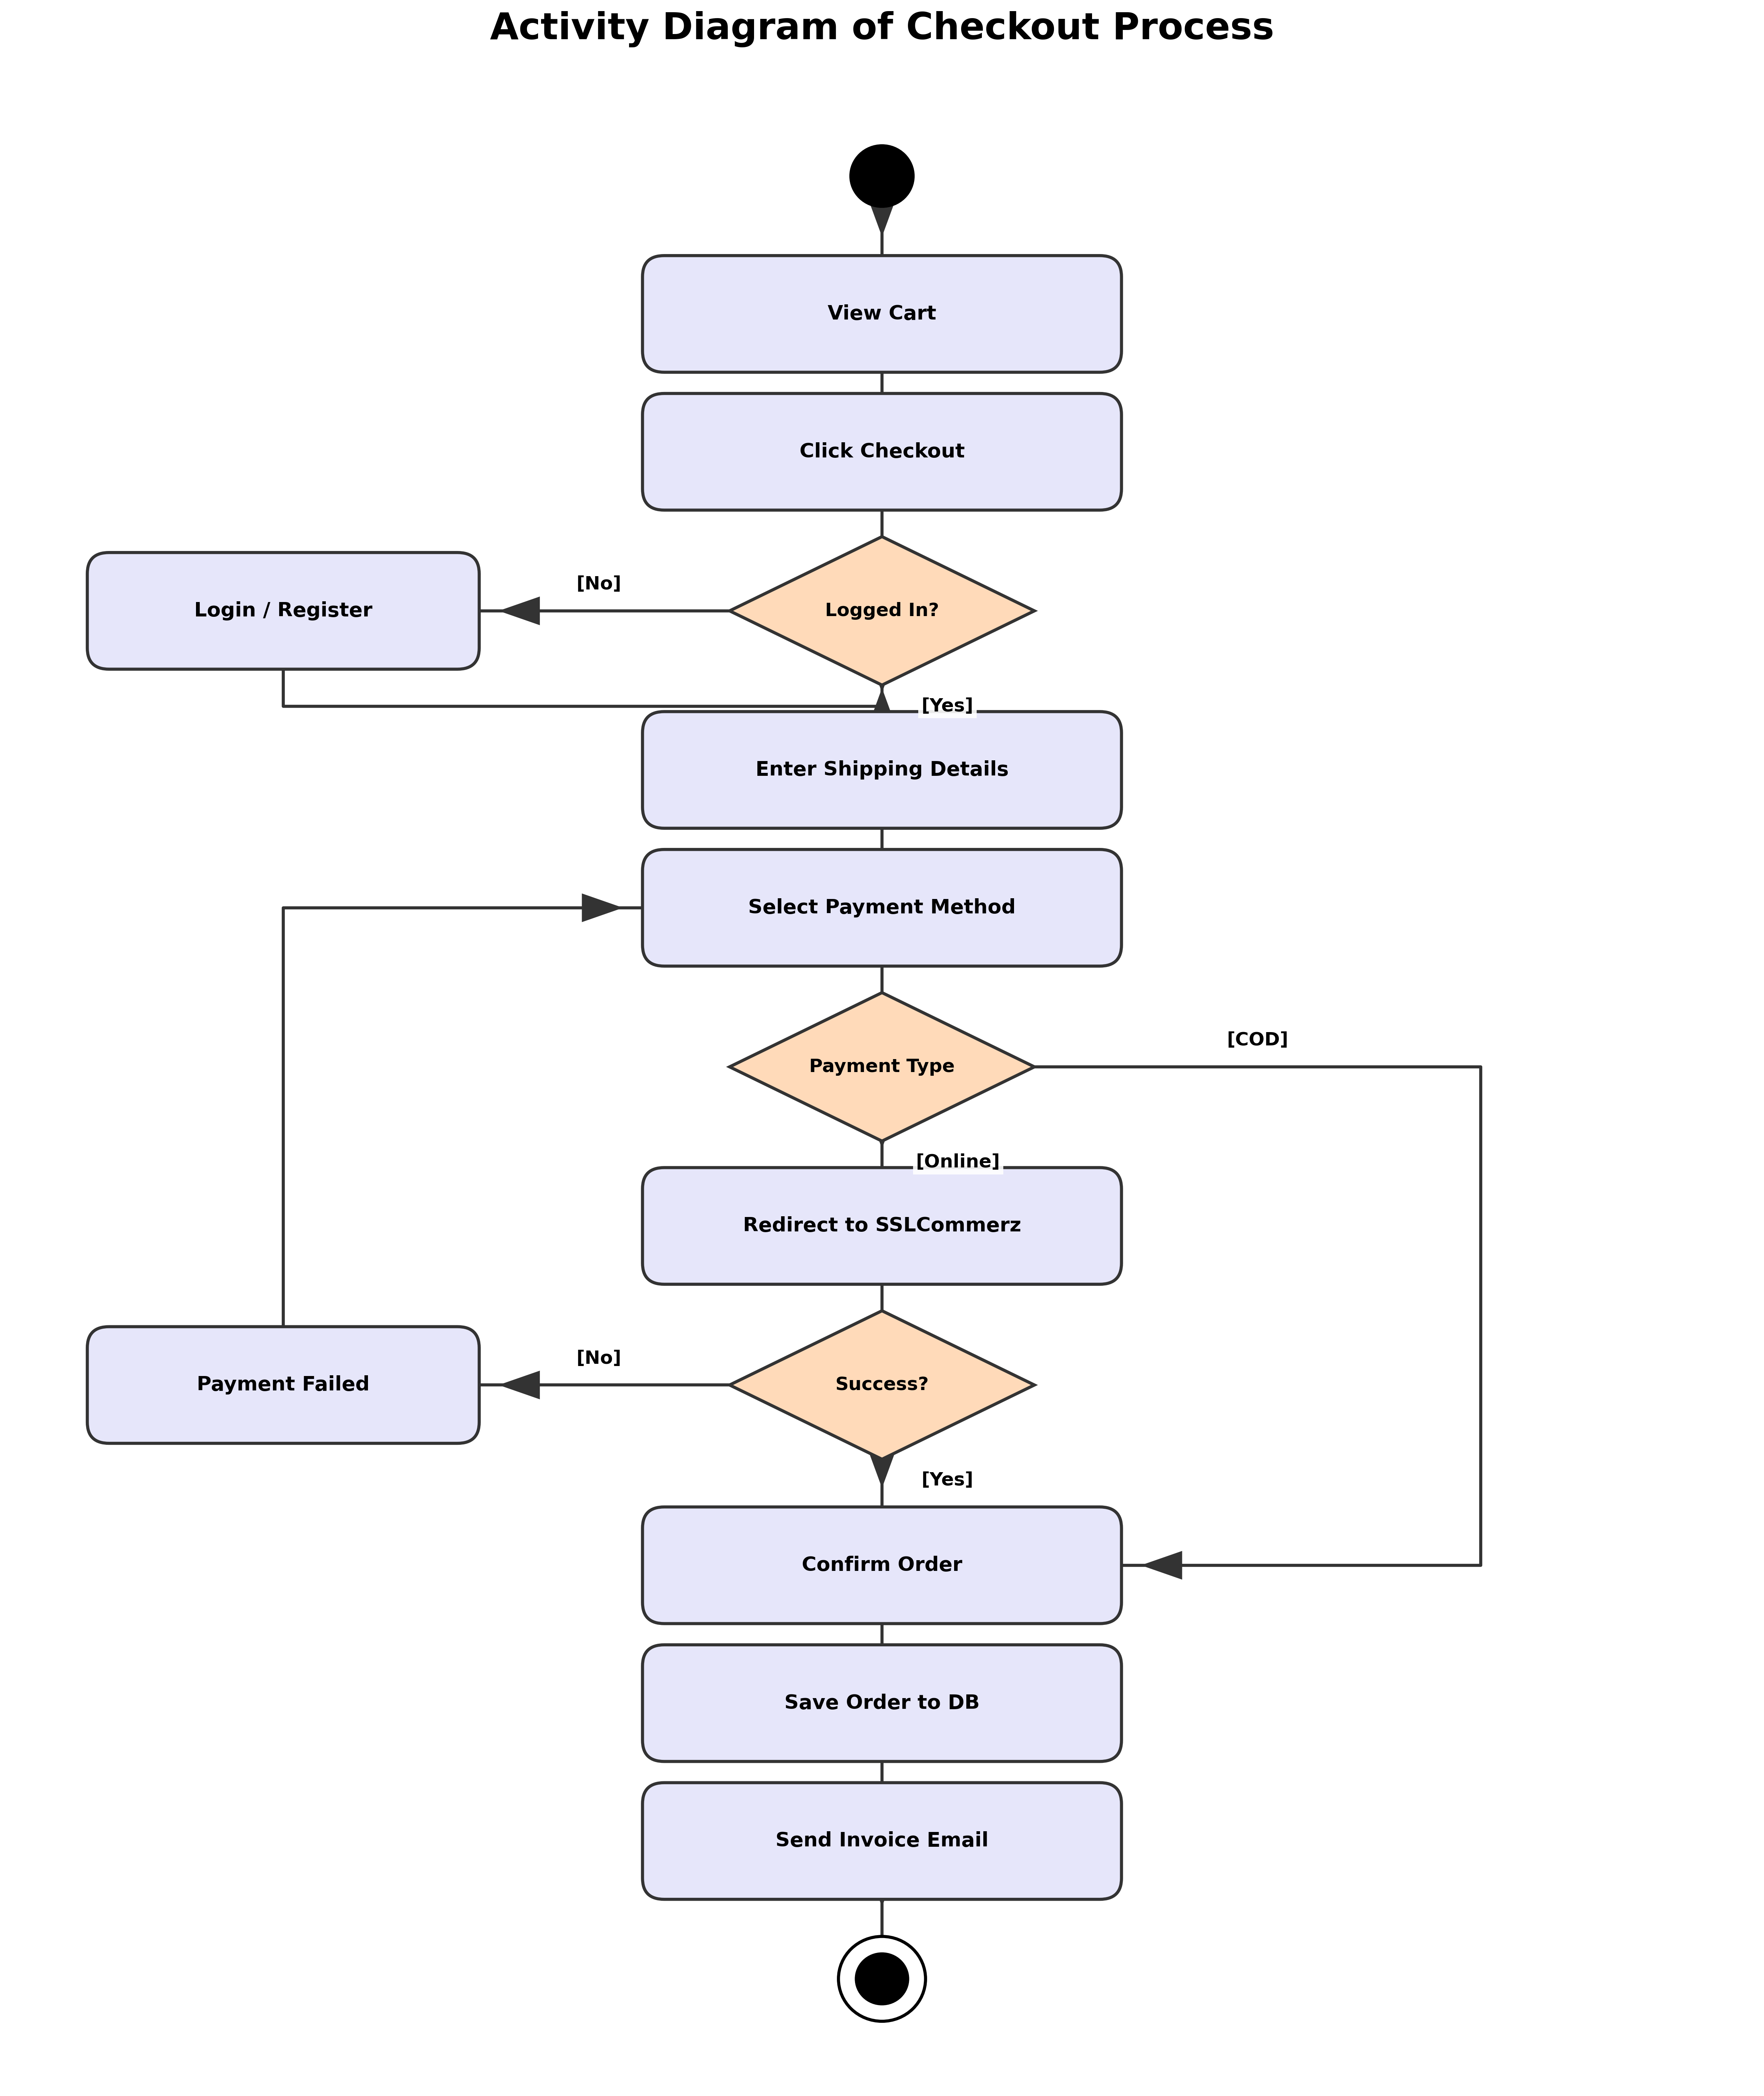
\includegraphics[width=\textwidth]{images/activity_diagram.png}
\caption{Activity Diagram of Checkout Process}
\end{figure}

\subsection{Sequence Diagram}
The Sequence Diagram details how objects interact in a particular scenario along a chronological timeline. This specific diagram explains the Payment Gateway Integration, showing the exact sequence of API calls exchanged between the Client browser, the GloBus Node.js Server, and the external SSLCommerz server to validate and complete a secure transaction.

\begin{figure}[h]
\centering
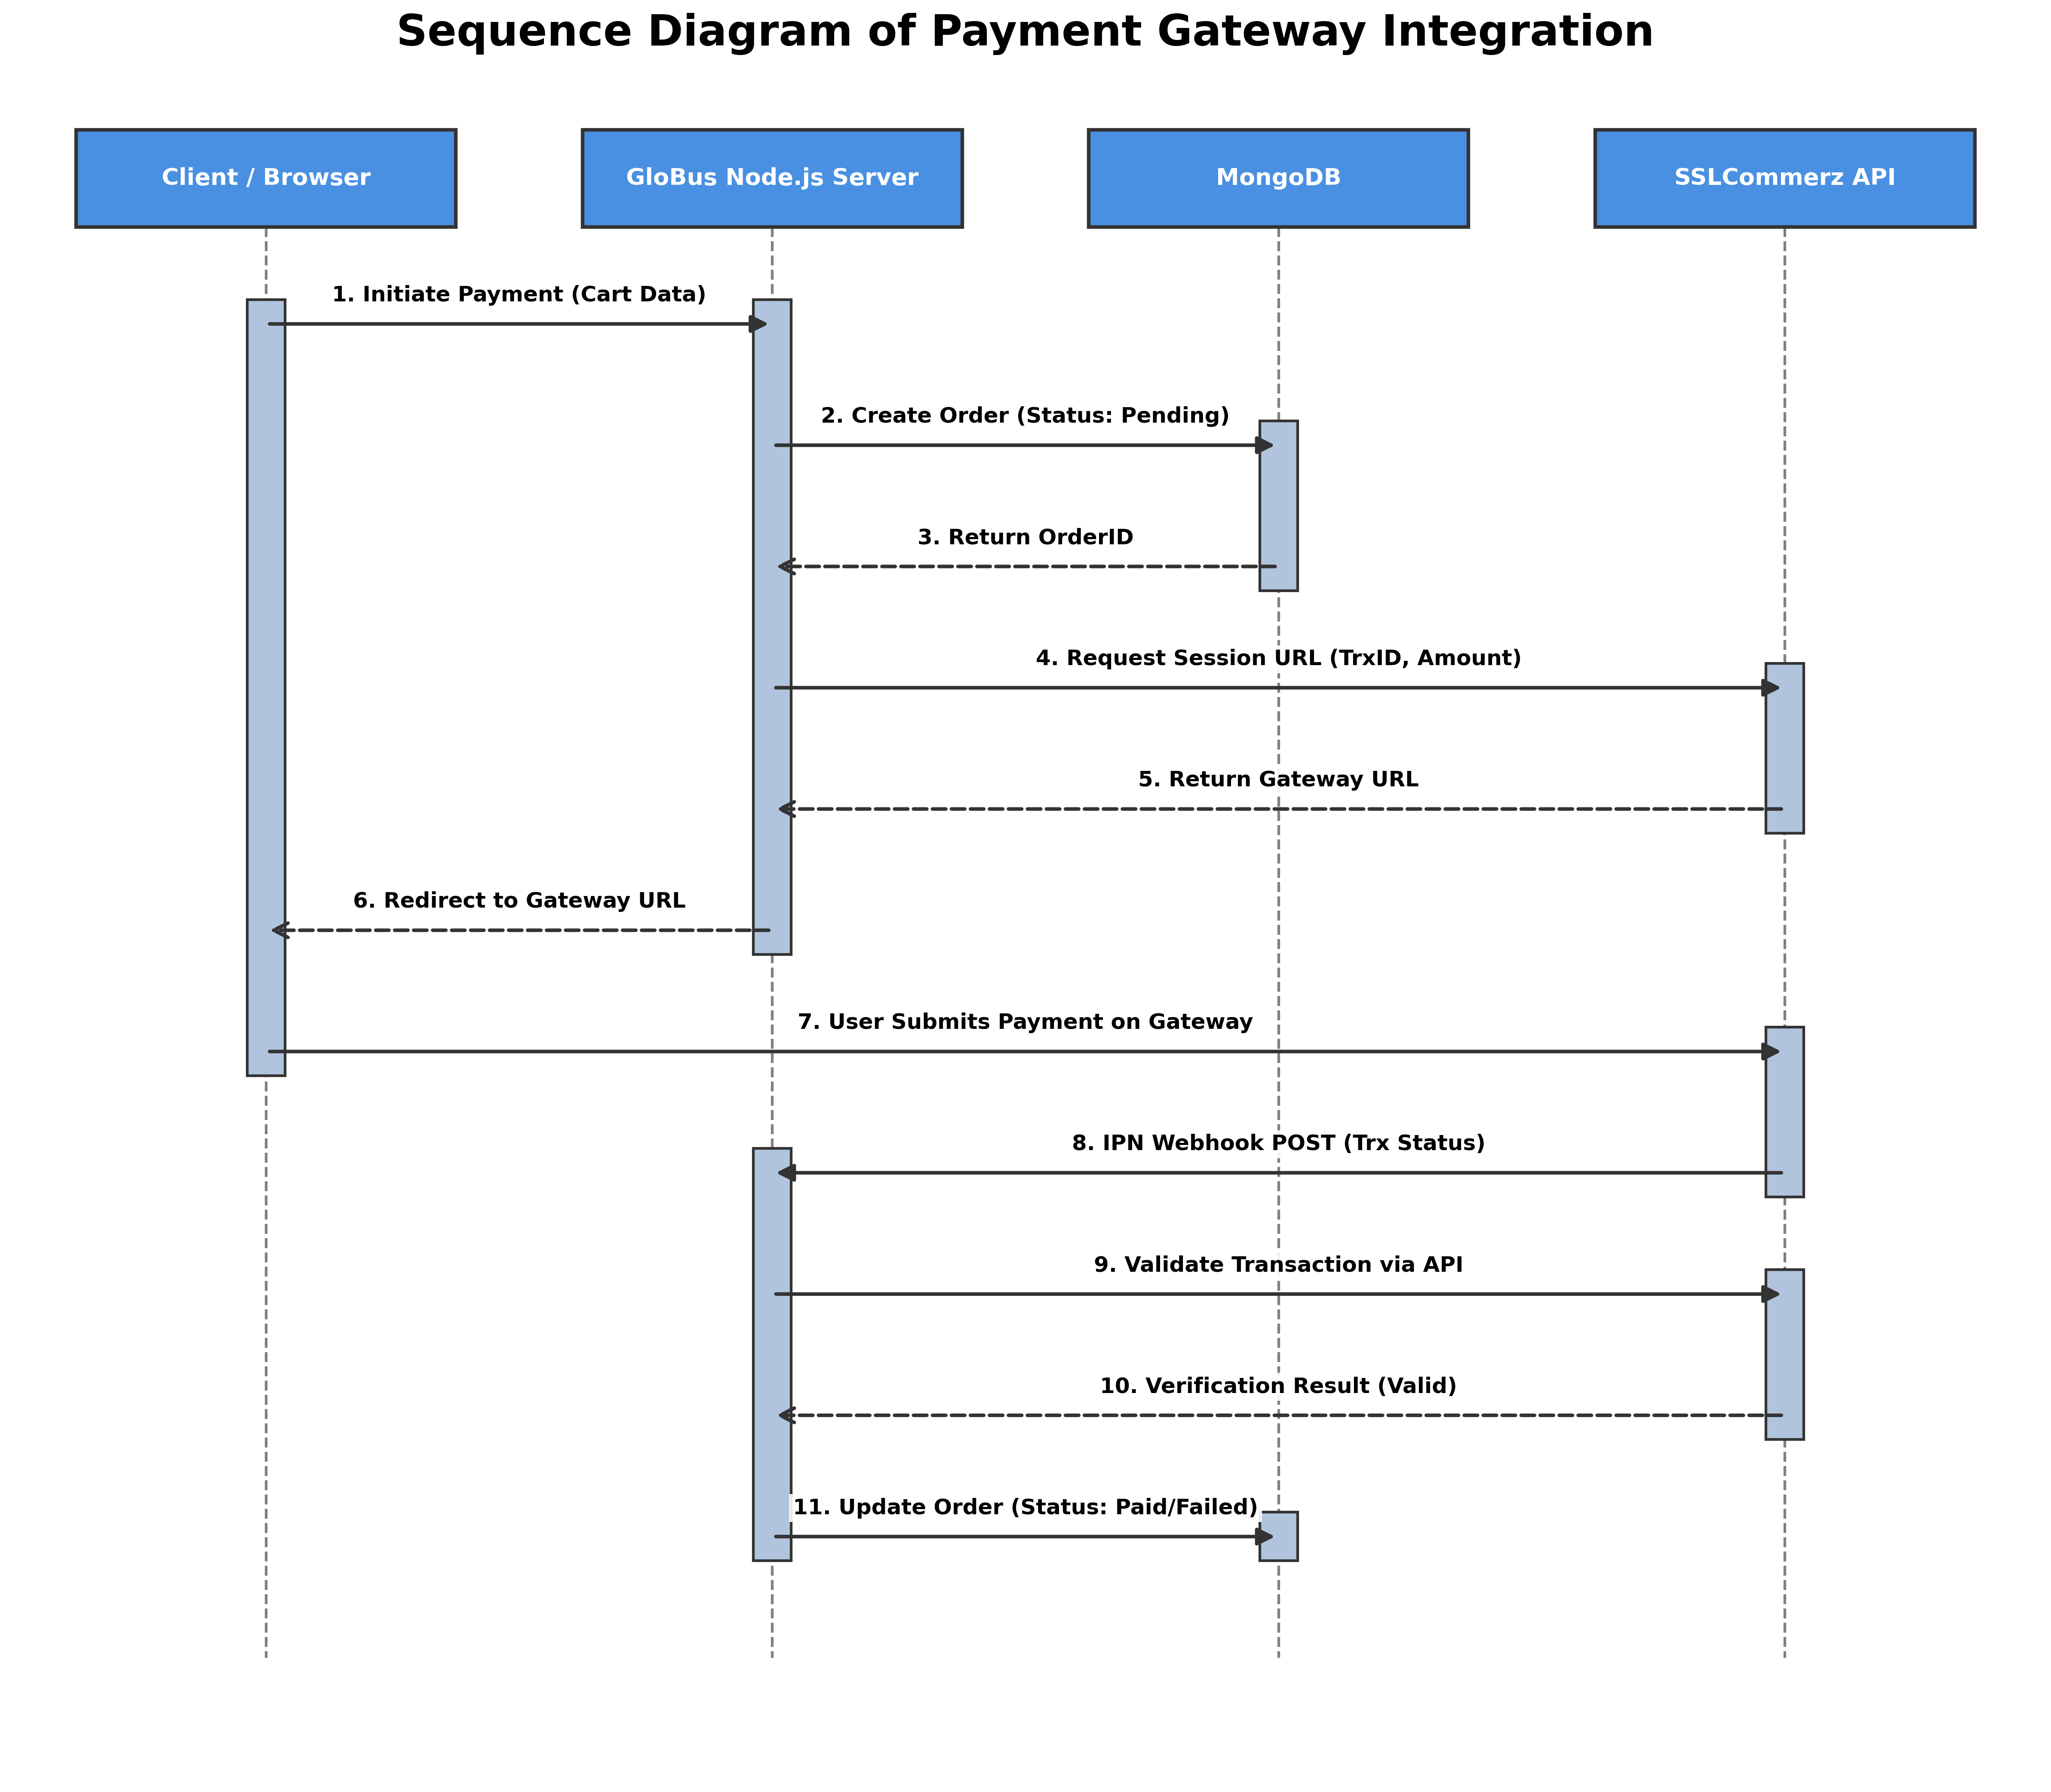
\includegraphics[width=\textwidth]{images/sequence_diagram.png}
\caption{Sequence Diagram of Payment Gateway Integration}
\end{figure}

\section{Feature Showcases}
The following figures demonstrate the core features and user interface of the GloBus platform.

\begin{figure}[h]
\centering
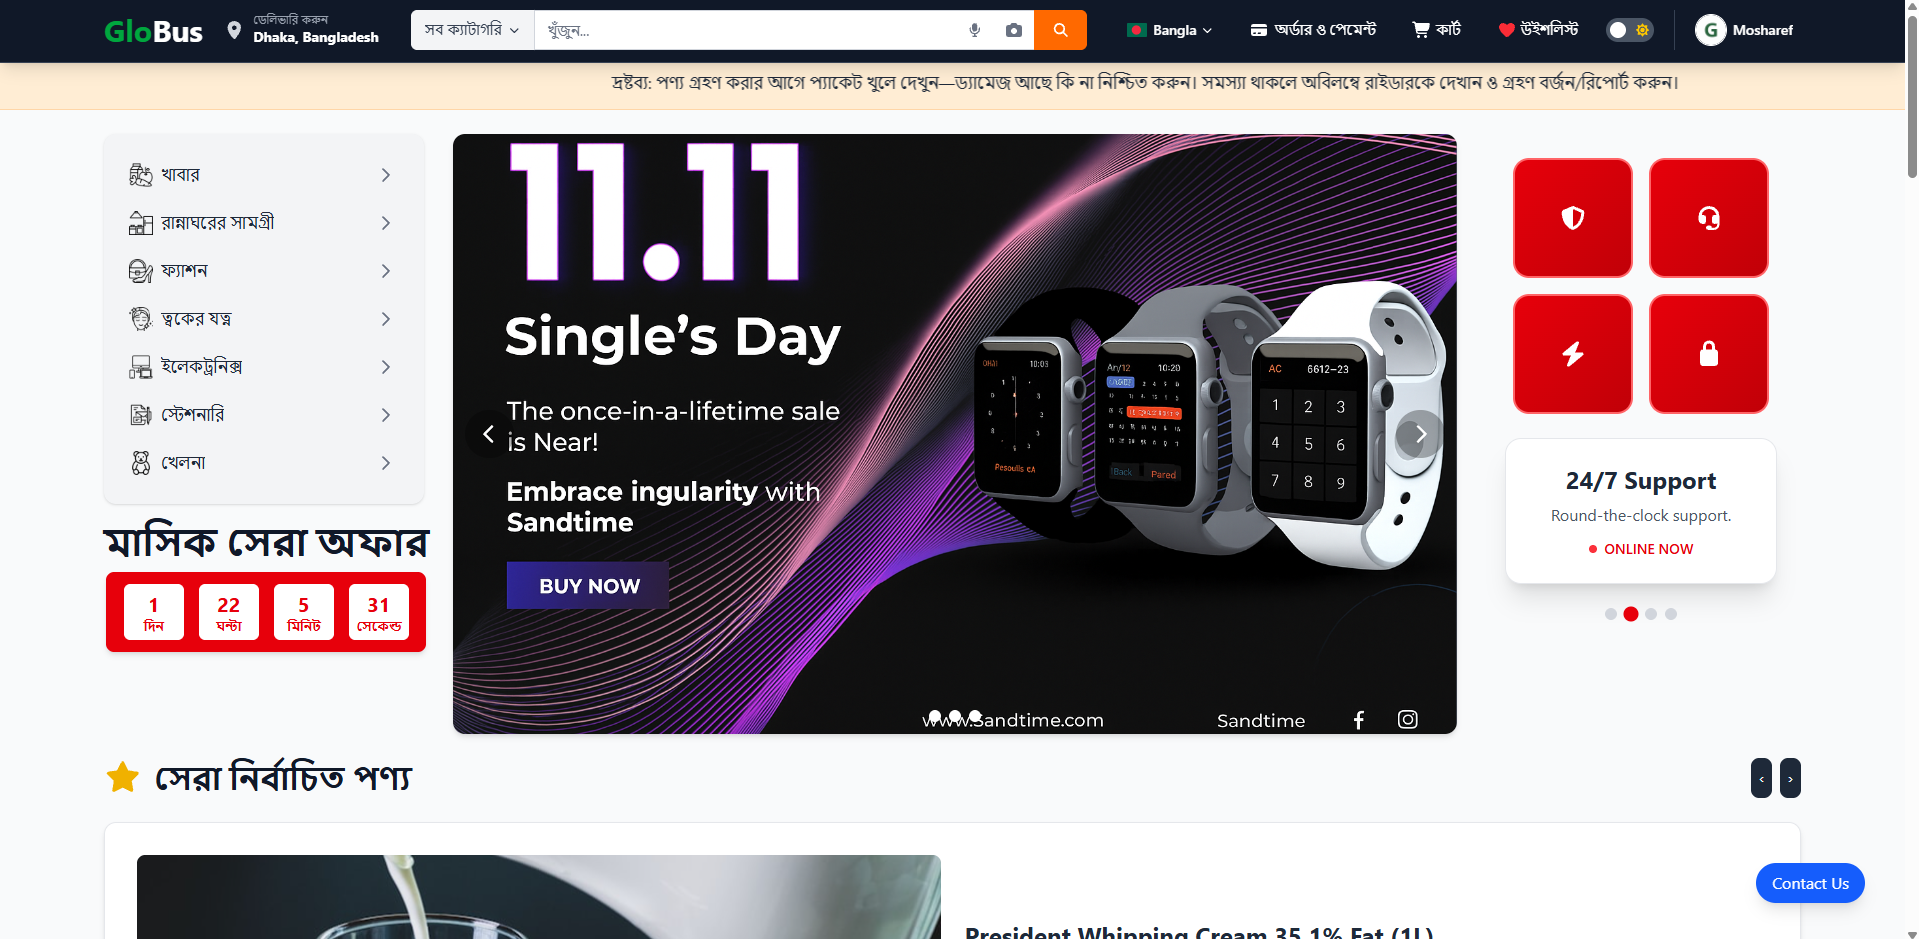
\includegraphics[width=\textwidth]{images/home_globus.png}
\caption{Feature: Home Page and Promotional Banner}
\end{figure}

\begin{figure}[h]
\centering
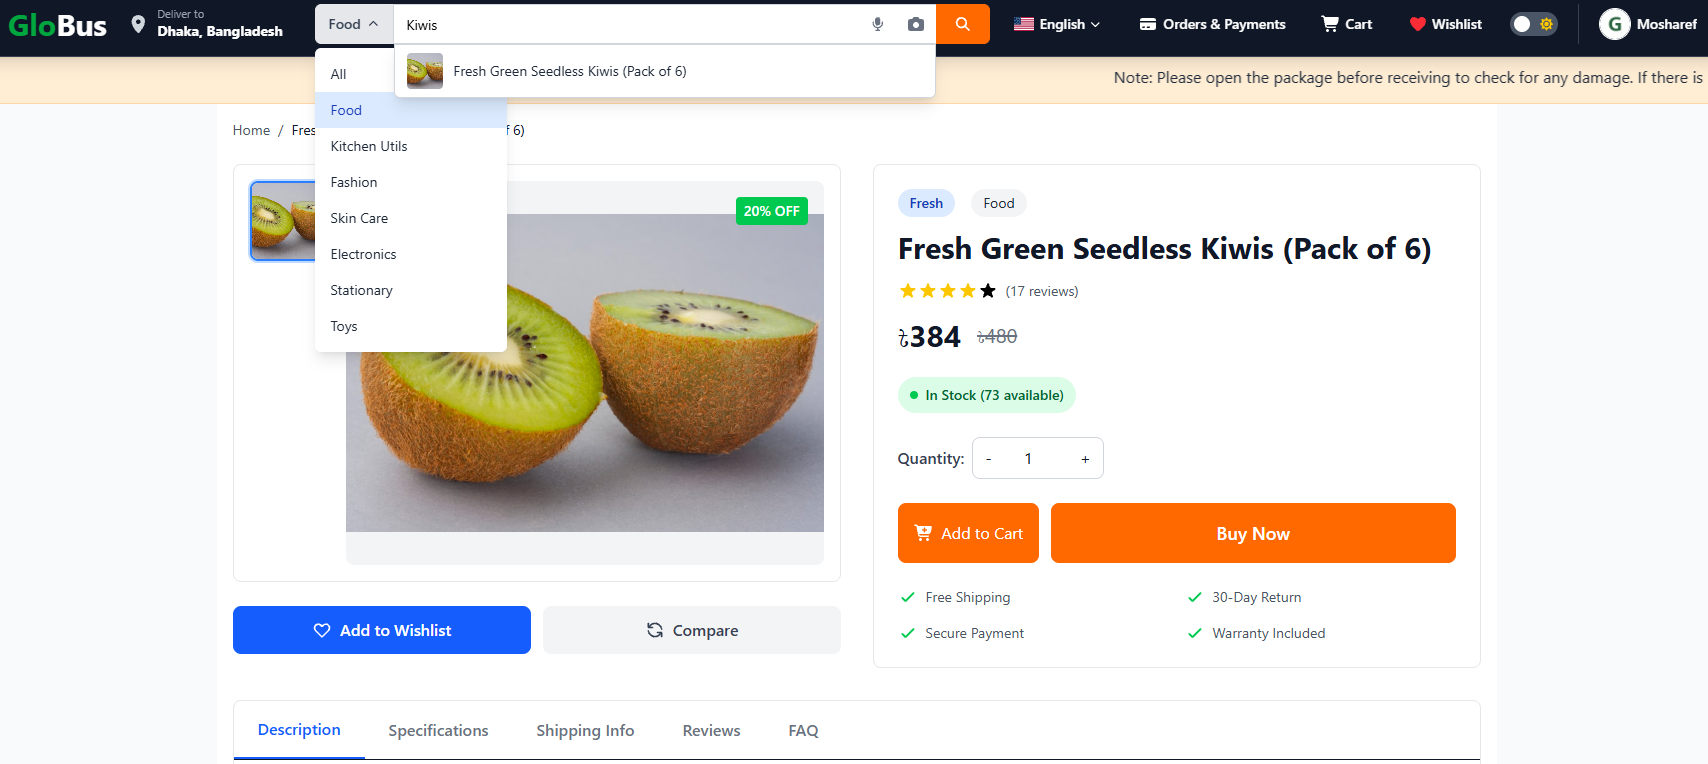
\includegraphics[width=\textwidth]{images/product_search.png}
\caption{Feature: Product Search and Categorized Browsing}
\end{figure}

\begin{figure}[h]
\centering
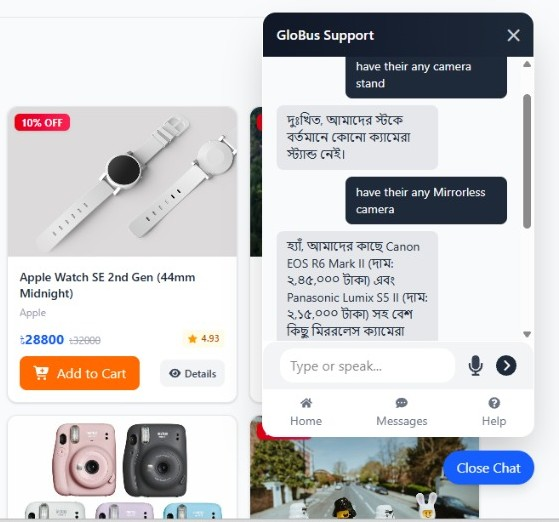
\includegraphics[width=\textwidth]{images/chat_ai.jpeg}
\caption{Feature: AI Vision Product Search}
\end{figure}

\begin{figure}[h]
\centering
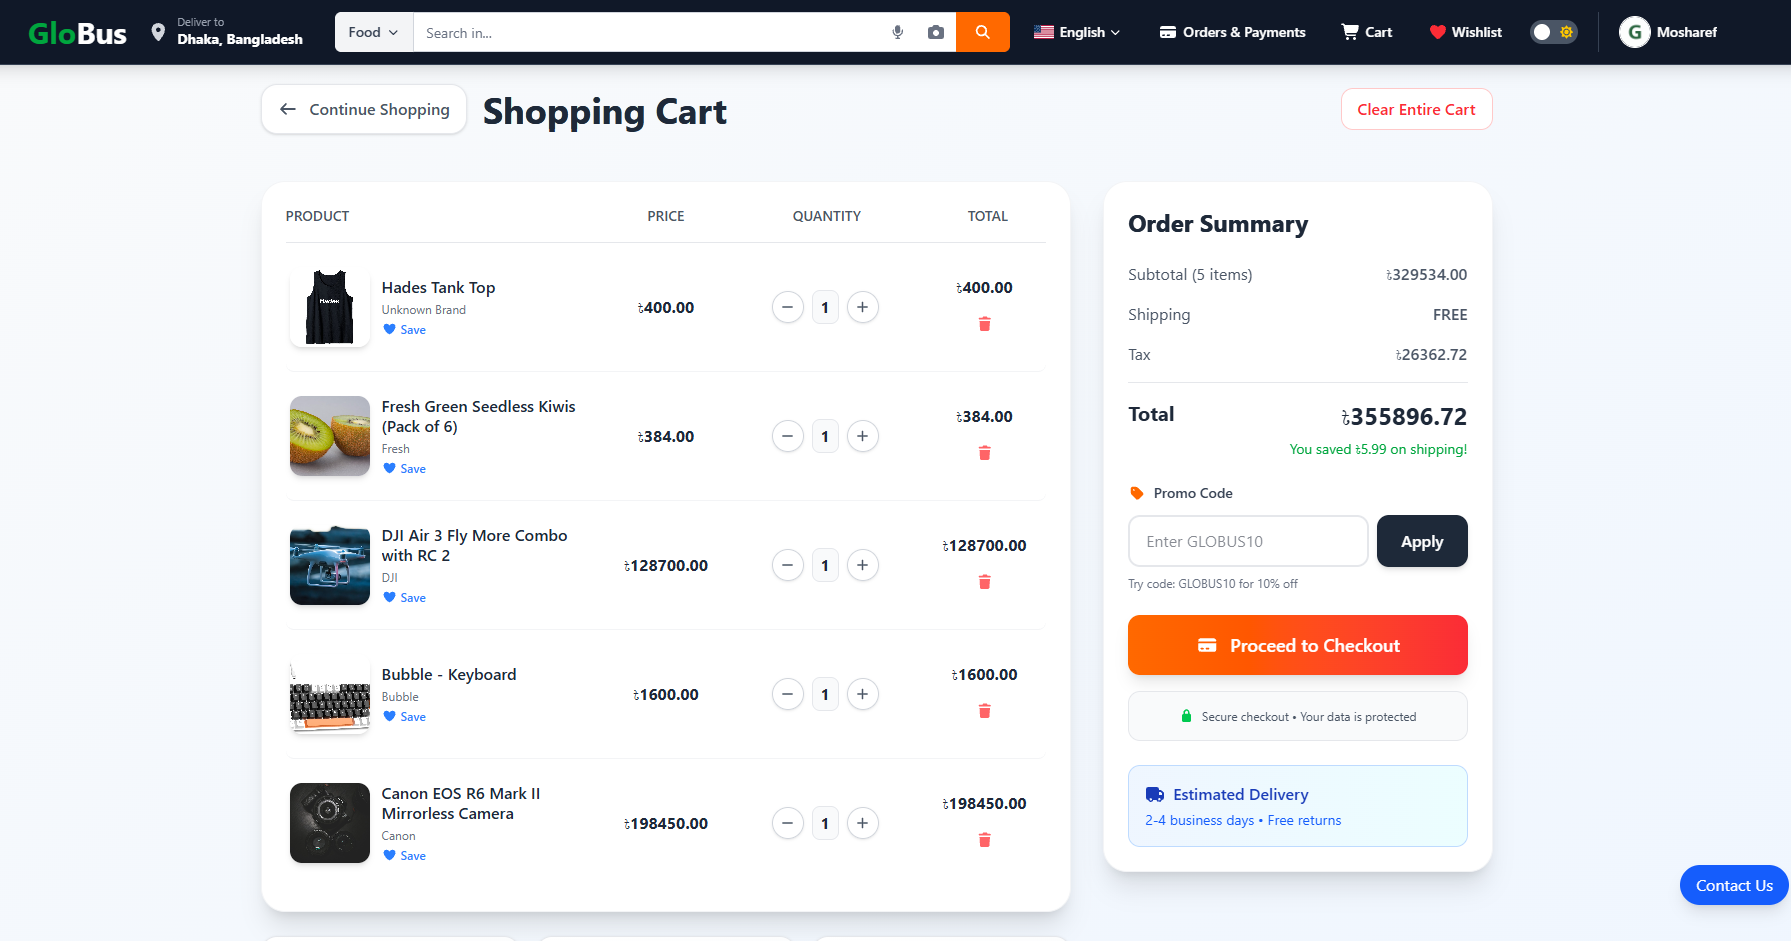
\includegraphics[width=\textwidth]{images/cart.png}
\caption{Feature: Interactive Shopping Cart}
\end{figure}

\begin{figure}[h]
\centering
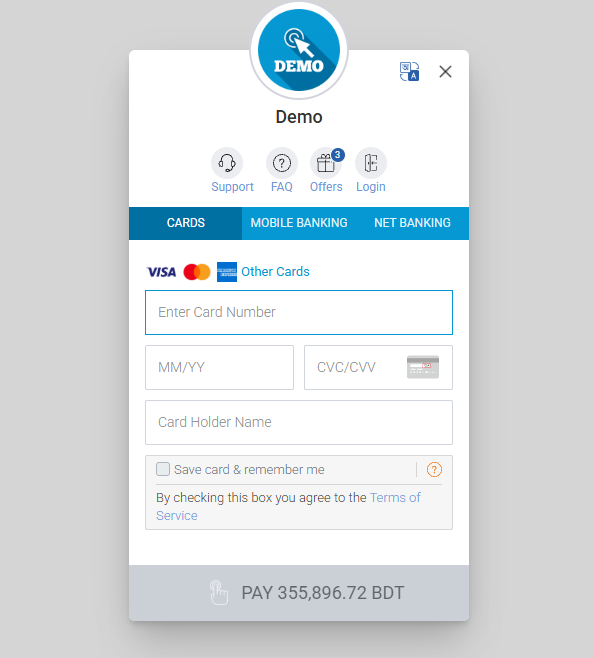
\includegraphics[width=\textwidth]{images/checkout.png}
\caption{Feature: Secure Checkout with SSLCommerz}
\end{figure}

\begin{figure}[h]
\centering
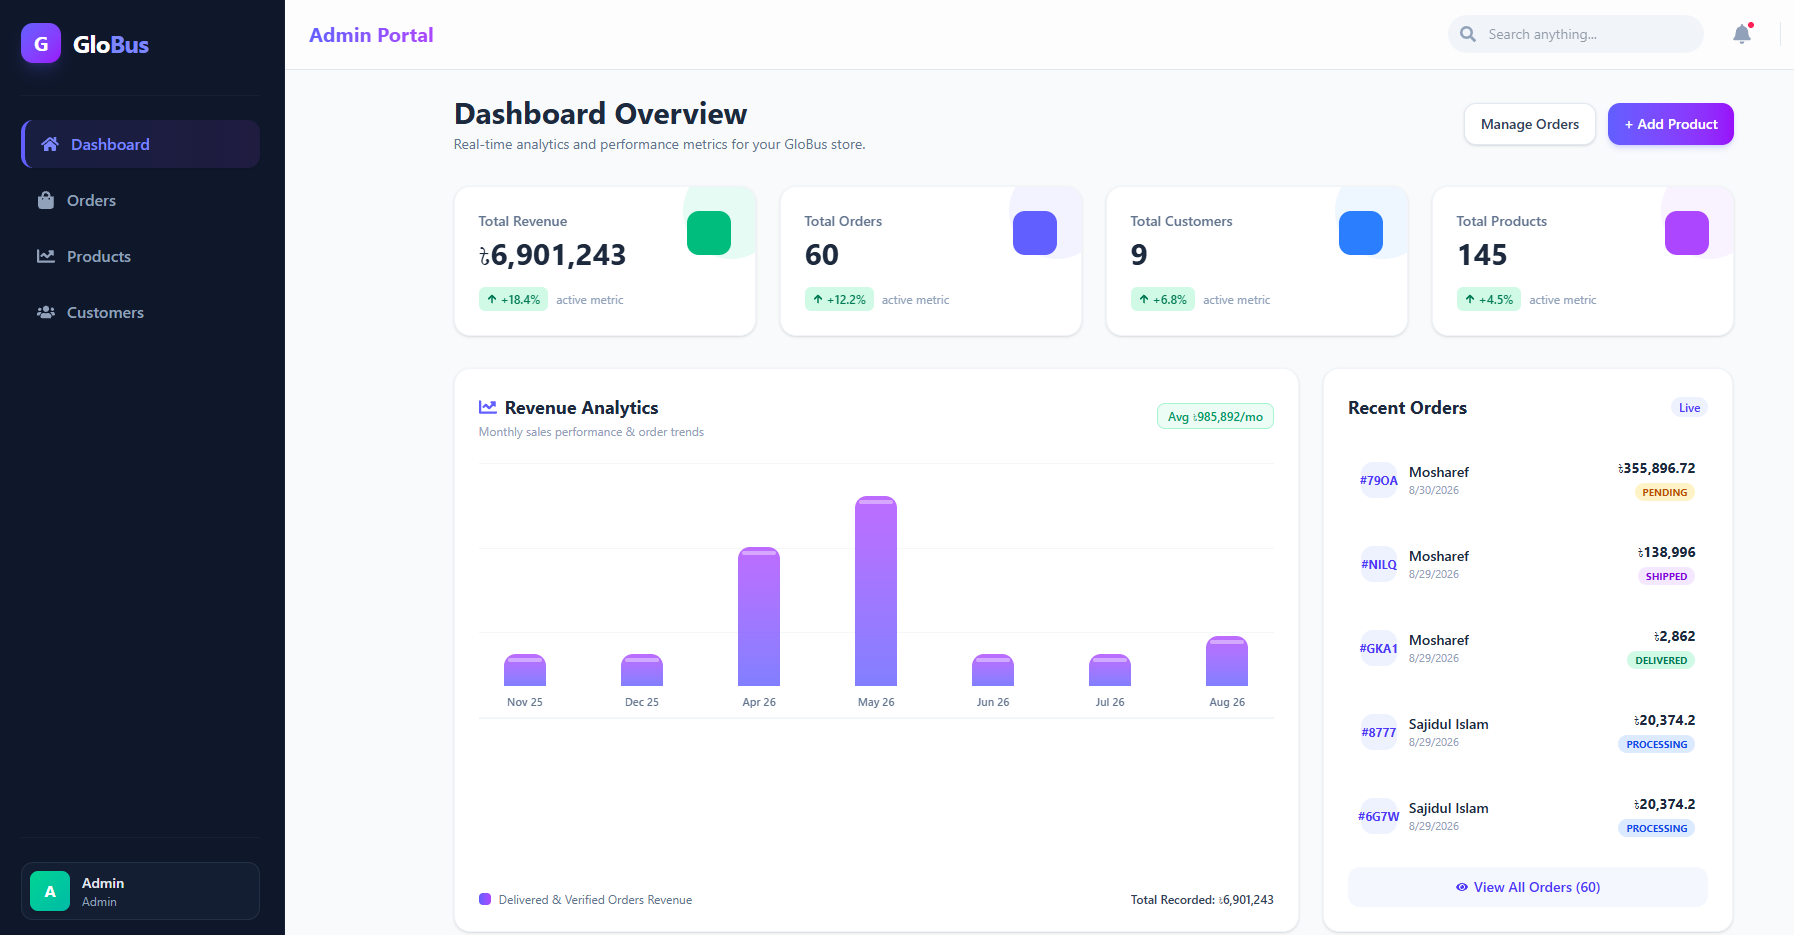
\includegraphics[width=\textwidth]{images/admin_dashboard_main.png}
\caption{Feature: Admin Dashboard - Statistics Overview}
\end{figure}

\begin{figure}[h]
\centering
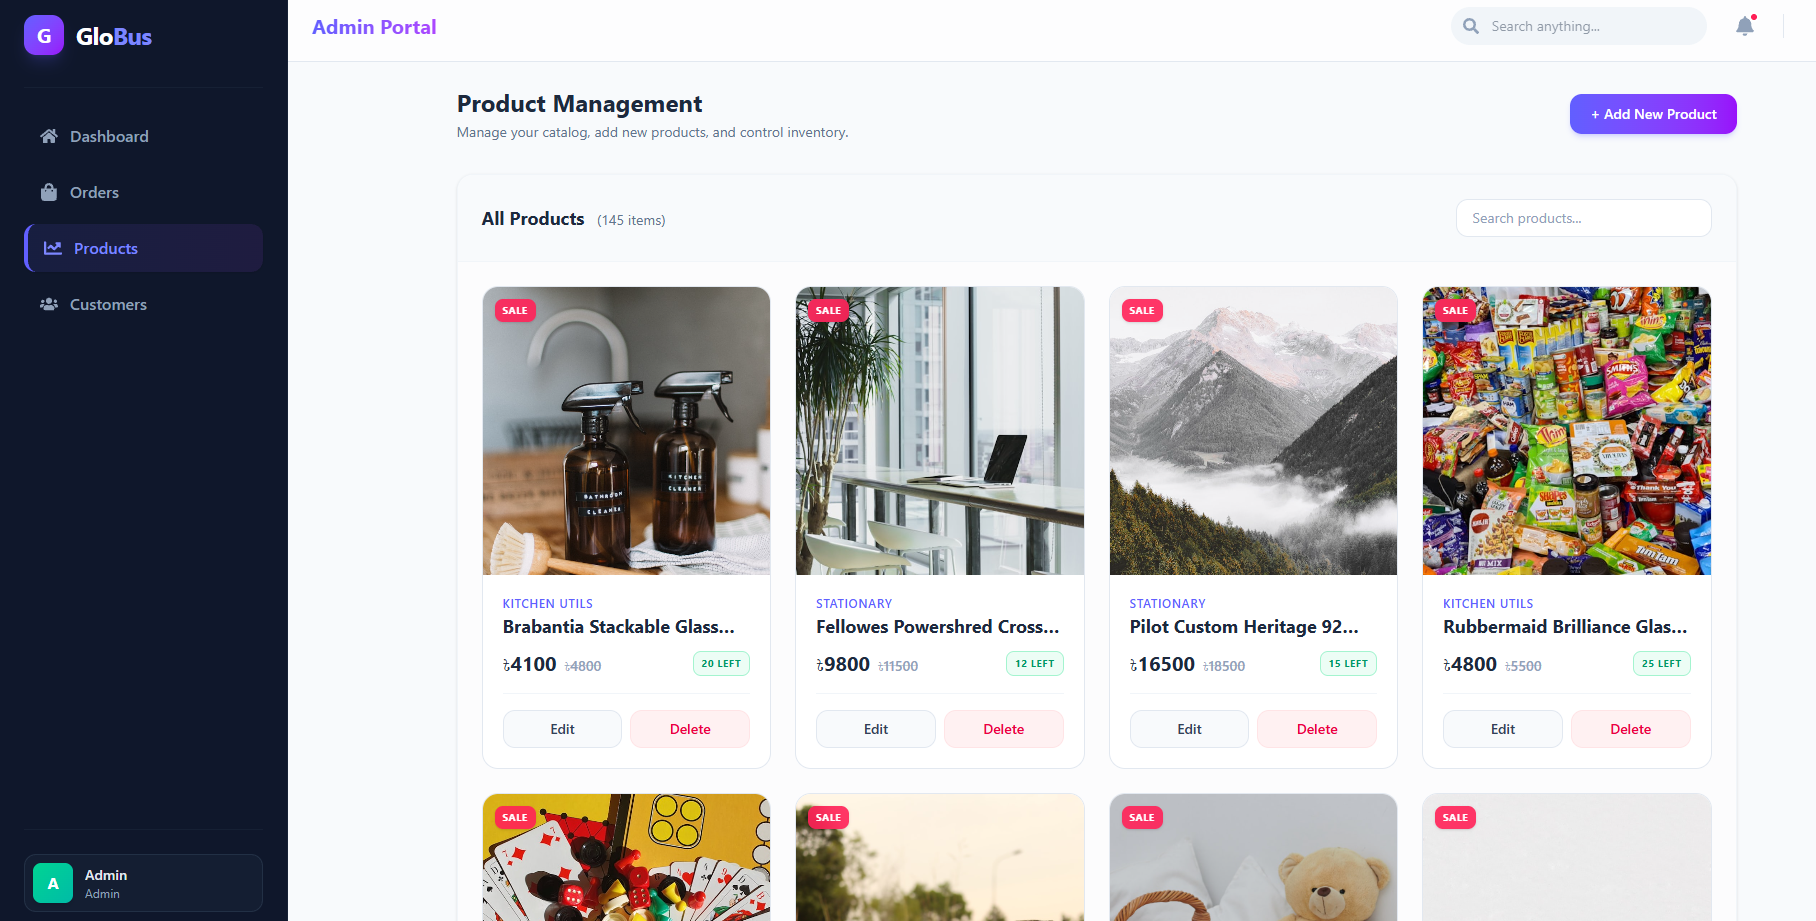
\includegraphics[width=\textwidth]{images/admin_dashboard_products.png}
\caption{Feature: Admin Dashboard - Product Management}
\end{figure}
